\documentclass[a4paper]{article}
\usepackage{vntex}
%\usepackage[english,vietnam]{babel}
%\usepackage[utf8]{inputenc}

%\usepackage[utf8]{inputenc}
%\usepackage[francais]{babel}
\usepackage{a4wide,amssymb,epsfig,latexsym,array,hhline,fancyhdr}

\usepackage{amsmath}
\usepackage{amsthm}
\usepackage{multicol,longtable,amscd}
\usepackage{diagbox}%Make diagonal lines in tables
\usepackage{booktabs}
\usepackage{alltt}
\usepackage[framemethod=tikz]{mdframed}% For highlighting paragraph backgrounds
\usepackage{caption,subcaption}

\usepackage{listings}
\usepackage{lastpage}
\usepackage[lined,boxed,commentsnumbered]{algorithm2e}
\usepackage{enumerate}
\usepackage{color}
\usepackage{graphicx}							% Standard graphics package
\usepackage{array}
\usepackage{tabularx, caption}
\usepackage{multirow}
\usepackage{multicol}
\usepackage{rotating}
\usepackage{graphics}
\usepackage{geometry}
\usepackage{setspace}
\usepackage{placeins}
\usepackage{epsfig}
\usepackage{tikz}
\usetikzlibrary{arrows,snakes,backgrounds}
\usepackage[unicode]{hyperref}
\hypersetup{urlcolor=blue,linkcolor=black,citecolor=black,colorlinks=true} 
%\usepackage{pstcol} 								% PSTricks with the standard color package

\newtheorem{theorem}{{\bf Định lý}}
\newtheorem{property}{{\bf Tính chất}}
\newtheorem{proposition}{{\bf Mệnh đề}}
\newtheorem{corollary}[proposition]{{\bf Hệ quả}}
\newtheorem{lemma}[proposition]{{\bf Bổ đề}}


%\usepackage{fancyhdr}
\setlength{\headheight}{40pt}
\pagestyle{fancy}
\fancyhead{} % clear all header fields
\fancyhead[L]{
 \begin{tabular}{rl}
    \begin{picture}(25,15)(0,0)
    \put(0,-8){
\includegraphics[width=8mm, height=8mm]{Images/hcmut.png}}
    %\put(0,-8){\epsfig{width=10mm,figure=hcmut.eps}}
   \end{picture}&
	%
\includegraphics[width=8mm, height=8mm]{hcmut.png} & %
	\begin{tabular}{l}
		\textbf{\bf \ttfamily Trường Đại Học Bách Khoa Tp.Hồ Chí Minh}\\
		\textbf{\bf \ttfamily Khoa Khoa Học và Kỹ Thuật Máy Tính}
	\end{tabular} 	
 \end{tabular}
}
\fancyhead[R]{
	\begin{tabular}{l}
		\tiny \bf \\
		\tiny \bf 
	\end{tabular}  }
\fancyfoot{} % clear all footer fields
\fancyfoot[L]{\scriptsize \ttfamily Bài tập lớn môn Mô hình hóa toán học (CO2011) - Niên khóa 2019-2020}
\fancyfoot[R]{\scriptsize \ttfamily Trang {\thepage}/\pageref{LastPage}}
\renewcommand{\headrulewidth}{0.3pt}
\renewcommand{\footrulewidth}{0.3pt}


%%%
\setcounter{secnumdepth}{4}
\setcounter{tocdepth}{3}
\makeatletter
\newcounter {subsubsubsection}[subsubsection]
\renewcommand\thesubsubsubsection{\thesubsubsection .\@alph\c@subsubsubsection}
\newcommand\subsubsubsection{\@startsection{subsubsubsection}{4}{\z@}%
                                     {-3.25ex\@plus -1ex \@minus -.2ex}%
                                     {1.5ex \@plus .2ex}%
                                     {\normalfont\normalsize\bfseries}}
\newcommand*\l@subsubsubsection{\@dottedtocline{3}{10.0em}{4.1em}}
\newcommand*{\subsubsubsectionmark}[1]{}
\makeatother

\everymath{\color{blue}}%make in-line maths symbols blue to read/check easily

\sloppy
\captionsetup[figure]{labelfont={small,bf},textfont={small,it},belowskip=-1pt,aboveskip=-9pt}
%space remove between caption, figure, and text
\captionsetup[table]{labelfont={small,bf},textfont={small,it},belowskip=-1pt,aboveskip=7pt}
%space remove between caption, table, and text

%\floatplacement{figure}{H}%forced here float placement automatically for figures
%\floatplacement{table}{H}%forced here float placement automatically for table
%the following settings (11 lines) are to remove white space before or after the figures and tables
%\setcounter{topnumber}{2}
%\setcounter{bottomnumber}{2}
%\setcounter{totalnumber}{4}
%\renewcommand{\topfraction}{0.85}
%\renewcommand{\bottomfraction}{0.85}
%\renewcommand{\textfraction}{0.15}
%\renewcommand{\floatpagefraction}{0.8}
%\renewcommand{\textfraction}{0.1}
\setlength{\floatsep}{5pt plus 2pt minus 2pt}
\setlength{\textfloatsep}{5pt plus 2pt minus 2pt}
\setlength{\intextsep}{10pt plus 2pt minus 2pt}

%phong
\definecolor{dkgreen}{rgb}{0,0.6,0}
\definecolor{gray}{rgb}{0.5,0.5,0.5}
\definecolor{mauve}{rgb}{0.58,0,0.82}
\lstset{frame=tb,
  language=R,
  aboveskip=3mm,
  belowskip=3mm,
  showstringspaces=false,
  columns=flexible,
  basicstyle={\small\ttfamily},
  numbers=none,
  numberstyle=\tiny\color{gray},
  keywordstyle=\color{blue},
  commentstyle=\color{dkgreen},
  stringstyle=\color{mauve},
  breaklines=true,
  breakatwhitespace=true,
  tabsize=3
}

\begin{document}

\begin{titlepage}
\begin{center}
ĐẠI HỌC QUỐC GIA THÀNH PHỐ HỒ CHÍ MINH \\
TRƯỜNG ĐẠI HỌC BÁCH KHOA \\
KHOA KHOA HỌC - KỸ THUẬT MÁY TÍNH 
\end{center}

\vspace{1cm}

\begin{figure}[h!]
\begin{center}

\includegraphics[width=3cm]{Images/hcmut.png}
\end{center}
\end{figure}

\vspace{1cm}


\begin{center}
\begin{tabular}{c}
\multicolumn{1}{l}{\textbf{{\Large MÔ HÌNH HÓA TOÁN HỌC ()}}}\\
~~\\
\hline
\\
\multicolumn{1}{l}{\textbf{{\Large Nhóm: ... ---- Bài tập lớn}}}\\
\\
\textbf{{\Huge Mô hình SIR}} \\
\textbf{{\Huge trong dự báo COVID-19}}\\
\\
\hline
\end{tabular}
\end{center}

\vspace{1.5cm}

\begin{table}[h]
\begin{tabular}{rrl}
\hspace{5 cm} & GVHD: & Nguyễn An Khương\\
\hspace{5 cm} &  & Huỳnh Tường Nguyên\\

& SV thực hiện: & Tăng Minh Nhật -- 1813380 \\
& & Đỗ Lê Thiên Ân -- 1810823 \\
& & Lê Hồng Phong -- 1813518 \\
& & Đặng Thành Ngân -- 1813187 \\
& & Huỳnh Thiên Trình -- 1810615 \\
\end{tabular}
\end{table}
\vspace{1.5cm}
\begin{center}
{\footnotesize Tp. Hồ Chí Minh, Tháng 7/2020}
\end{center}
\end{titlepage}


%\thispagestyle{empty}

\newpage
\tableofcontents
\newpage

Bài báo cáo này trình bày lời giải một số bài toán về thống kê mô tả và mộ số bài toán liên quan đến các mô hình xác suất rời rạc có sử dụng R.

Trong phần đầu, chúng tôi nhắc lại một số kiến thức và kết quả cơ bản về thống kê mô tả, và các mô hình xác suất rời rạc thông dụng, cùng với một số hàm R thông dụng mà chúng tôi sử dụng để tính toán kết quả trong các lời giải của các bài toán trong Phần \ref{bai_tap}.

Đối với mỗi bài toán Phần \ref{bai_tap}, trước hết chúng tôi trình bày lời giải truyền thống, bằng cách dùng các công thức và kết quả đã được trình bày trong Phần~\ref{chuan_bi}. Sau đó chúng tôi tính toán lại kết quả bằng các hàm R. Các biểu đồ (nếu có) cũng sẽ được vẽ bằng R và nhúng vào LaTeX.

%%%%%%%%%%%%%%%%%%%%%%%%%%%%%%%%%
\section{Kiến thức chuẩn bị}\label{chuan_bi}
\subsection{Tổng quan về R và Python} 
...
\subsection{Phương pháp xấp xỉ Euler trong giải hệ phương trình vi phân.}
Phương pháp Euler là một phương pháp bậc một thường được sử dụng trong việc giải các
phương trình vi phân thường. Phương pháp được đặt tên theo Leonhard Euler, người đã giới
thiệu phương pháp trong quyển sách Institutionum Calculi Integralis cùng tên xuất bản trong
khoảng thời gian 1768 đến 1770.\\

Xem xét bài toán tính toán hình dạng của một đường cong chưa biết bắt đầu tại một điểm cho trước và thỏa mãn một phương trình vi phân nào đó. Ở đây, phương trình vi phân có thể được coi như là một công thức mà nhờ nó độ dốc của đường tiếp tuyến với đường cong có thể được tính toán tại điểm bất kỳ nào trên đường cong, một khi vị trí của điểm đó đã được tính toán.\\

Ý tưởng là trong khi đường cong ban đầu chưa biết, điểm khởi đầu của nó được biểu thị bởi $A_{0}$ là đã biết (xem hình phía trên bên phải). Thì, từ phương trình vi phân, độ dốc của đường cong tại có thể được tính toán, và vì vậy, có thể tìm được đường tiếp tuyến.\\

Đi một bước nhỏ dọc theo đường tiếp tuyến đến một điểm $A_{1}$ Dọc bước nhỏ này, độ dốc không thay đổi quá nhiều, vì vậy $ A_{1}$ sẽ gần với đường cong. Nếu chúng ta coi $A_{1}$ vẫn còn nằm trên đường cong, cùng một lý luận như đối với điểm $A_{0}$ có thể tính được độ dốc và tiếp tuyến của đường cong tại $A_{1}$. Sau vài bước, một đường cong đa giác $ A_{0}A_{1}A_{2}A_{3}$... được tìm ra. Nói chung, đường cong này không phân kỳ quá xa khỏi đường cong chưa biết ban đầu, và sai số giữa hai đường cong có thể được làm nhỏ nếu kích thước bước là đủ nhỏ và khoảng thời gian tính toán là hữu hạn\\
  \begin{figure}[htp]
	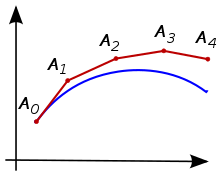
\includegraphics[height=6cm]{Images/Euler_method.png}
	\centering
	\caption{Minh họa phương pháp Euler. Đường cong chưa biết có màu xanh da trời và lời giải gần đúng của nó là đường nhiều cạnh màu đỏ.}
	\centering
	\end{figure}
	\FloatBarrier

Giả sử ta có phương trình vi phân bậc nhất
\begin{center}
    $ y'(t)=f(t,y(t)),\qquad \qquad y(t_{0})=y_{0}$
\end{center}

Trên đoạn [a,b] ta chia thành n đoạn bằng nhau với\\
\begin{center}
    $\Delta t = \frac{b-a}{n}$ 
\end{center}
$\Delta t$ là kích thước của mỗi bước và đặt $t_{n}=t_{0}+n\Delta t$. Xét phương trình vi phân $y'(t)=f(t,y(t))$. Phương pháp Euler thuận thu được bằng cách sử dụng sai phân xấp xỉ thuận
\begin{center}
    $\frac{y_{n+1}-y{n}}{\Delta t}\approx y'(t)=f(t,y(t))$
    =>$y_{n+1}=y_{n}+f(t,y(t))\Delta t.$
\end{center}

Ở dạng tổng quát, một hệ phương trình vi phân bậc một được viết dưới dạng\\
    $\qquad \qquad y_{1}=y_{0}+f(t_{0},y(t_{0}))\Delta t.$\\
    $\qquad \qquad y_{2}=y_{1}+f(t_{1},y(t_{1}))\Delta t.$\\
    $\qquad \qquad ...$\\
    $\qquad \qquad y_{n}=y_{n-1}+f(t_{n-1},y(t_{n-1}))\Delta t.$\\

      \begin{figure}[htp]
	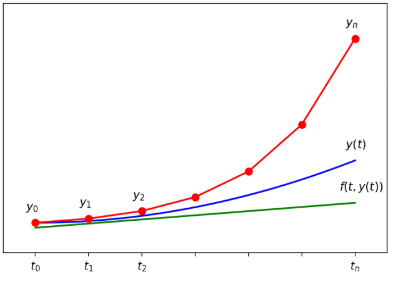
\includegraphics[height=6cm]{Images/euler.png}
	\centering
	\caption{Các điểm tròn màu đỏ chính là giá trị xấp xỉ đường cong $y$ có độ dốc  $ y'(t)=f(t,y)$ nghĩa là $y'=f(t,y)$. Sai khác giữa $y_{n}$ và $y_{n-1}$ đúng bằng $f(t_{n-1},y_{n-1})(t_{n}-t_{n-1})$ } 
	\centering
	\end{figure}
	\FloatBarrier
trong đó $y_{i}$ là các hàm số thực phụ thuộc vào biến $ t\geq 0$ và $f_{i}$ là các hàm số thực phi tuyến phụ thuộc vào biến $t \geq 0$ và các $ y_{i}$’s với mọi $i \in {1, . . . , N}$. Phương pháp Euler khi đó được áp dụng cho từng $y_{i}$.\\
\subsection{Giải thuật Metropolis-Hastings}
\subsubsection{Phương pháp Monte Carlo}
\subsubsubsection{Sơ lược}
Các phương pháp Monte Carlo là một lớp các thuật toán để giải quyết nhiều bài toán trên máy tính theo kiểu không tất định, thường bằng cách sử dụng các số ngẫu nhiên (thường là các số giả ngẫu nhiên), ngược lại với các thuật toán tất định
\subsubsubsection{Phương pháp chung}
Phương pháp Monte Carlo có thể có nhiều biến thể khác nhau, nhưng thường sẽ theo các bước sau: 
\begin{itemize}
    \item Bước 1: Chọn miền xác định các biến đầu vào
    \item Bước 2: Chọn các biến đầu vào, thuộc miền xác định, 1 cách ngẫu nhiên dựa trên 1 hàm phân phối xác suất trên miền xác định đã chọn ở câu 1
    \item Bước 3: Thực hiện 1 phép tính toán tất định trên các biến đầu vào đó
    \item Bước 4: Tổng hợp kết quả
\end{itemize}

\subsubsection{Sơ lược về xích Markov}
\subsubsubsection{Quá trình Markov}
Quá trình Markov là một quá trình ngẫu nhiên, mà dự đoán về các trạng thái trong tương lai của nó phụ thuộc hoàn toàn vào trạng thái hiện tại, và dự đoán này chính xác như là nếu ta đã biết toàn quá trình trong tương lai lẫn quá khứ, nói cách khác, trạng thái trong quá khứ và tương lai là độc lập đôi một với nhau
\subsubsubsection{Xích Markov}
Xích Markov thường được định nghĩa là 1 quá trình Markov mà không gian trạng thái, hoặc tập index (thường sử dụng thời gian), là rời rạc 
\subsubsubsection{Xích Markov Monte Carlo (MCMC)}
MCMC  là một họ gồm nhiều thuật toán thường dùng để lấy mẫu phân bố xác suất nhiều chiều dựa trên việc xây dựng xích Markov có phân bố dừng tương ứng và kỹ thuật gieo điểm ngẫu nhiên Monte Car.
Bằng cách xây dựng 1 xích Markov với phân phối mong muốn là phân phối cân bằng, ta có thể lấy mẫu của phân phối mong muốn đó bằng cách ghi lại các trạng thái từ xích. Có nhiều phương thức để xây dựng chuỗi, một trong số đó là giải thuật Metropolis-Hastings.
\subsubsection{Giải thuật Metropolis-Hastings}
\subsubsubsection{Phương pháp}
Thuật toán Metropolis–Hastings được biết đến là một phương pháp xích Markov Monte Carlo có các bước như sau:
\begin{enumerate}
    \item  Khởi tạo $\beta_0$ và $\gamma_0$ từ phân bố xác suất tiên nghiệm $\pi(\beta,\gamma)$
    \item  Gán $\beta:=\beta_0$ và $\gamma:=\gamma_0$
    \item Khởi tạo  $\beta^*$ và $\gamma^*$ ngẫu nhiên từ phân phối xác suất bất kỳ $p(\beta,\gamma)$
    \item Nếu  $p(\beta,\gamma)$ là đối xứng, nghĩa là $p(\beta^*,\gamma^*|\beta,\gamma) = p(\beta,\gamma|\beta^*,\gamma^*)$, gán cho $r$ là xác suất giữ lại $\beta^*$ và $\gamma^*$ bằng công thức:
    \begin{align} 
        &r := min(1,\frac{\pi(\beta^*,\gamma^*)}{\pi(\beta,\gamma)})
	\end{align}
	và đi đến bước 6
	\item Nếu không đối xứng, gán
    \begin{align} 
        &r := min(1,\frac{\pi(\beta^*,\gamma^*)p(\beta,\gamma|\beta^*,\gamma^*) }{\pi(\beta,\gamma)p(\beta^*,\gamma^*|\beta,\gamma)})
	\end{align}
	\item  Khởi tạo giá trị $q$ ngẫu nhiên từ phân phối đều liên tục $U(0,1)$ .
	\item Nếu $q < r$, tạo $\beta_{i+1}:=\beta^*$ và $\gamma_{i+1}:= \gamma^*$ với i là chỉ số phần tử trong mẫu và đi đến bước 9.
    \item Ngược lại, tạo $\beta_{i+1} := \beta_i$ và $\gamma_{i+1} := \gamma_{i}$ và đi đến bước 9
    \item Lặp lại từ bước 2 với $\beta := \beta_{i}$ và $\gamma := \gamma_{i}$ cho đến khi đủ kích cỡ mẫu.
\end{enumerate}
\subsection{Một số kiến thức khác về xác suất và thống kê}

\subsubsection{Xác suất tiên nghiệm}
Xác suất tiên nghiệm trong tiếng anh là Priori Probability

Xác suất tiên nghiệm là một phương pháp dự đoán khả năng một biến cố sẽ xuất hiện theo một cách nhất định dựa trên tỉ lệ phần trăm, chứ không phải được xác định từ dữ liệu lịch sử. 

Nói cách khác, xác suất tiên nghiệm nhìn vào tính logic hơn là dữ liệu trong quá khứ để xác định xác suất một biến cố có thể xảy ra.   

Đặc điểm của Xác suất tiên nghiệm 
Xác suất tiên nghiệm thường được sử dụng trong phương pháp tính toán xác suất. 

Điều này là do người quan sát phải sử dụng logic để xác định các kết quả có thể xảy ra của một biến cố để xác định các hình thức mà các kết quả này có thể xảy ra.

Xác suất tiên nghiệm thường được sử dụng để xác định khả năng xảy ra các biến cố độc lập ở đó khả năng xảy ra một biến cố nhất định sẽ không bị ảnh hưởng bởi các biến cố đã xảy ra trước đó.

Xác suất tiên nghiệm có thể được áp dụng cho tất cả các trò chơi ngẫu nhiên như roullette, ném xúc xắc, chơi xổ số, v.v.

Hạn chế lớn nhất của phương pháp xác định xác suất này là nó chỉ có thể được áp dụng cho một tập hợp các biến cố hữu hạn vì hầu hết các biến cố đều có xác suất có điều kiện.


\subsubsection{Xác xuất hậu nghiệm}
Xác suất hậu nghiệm trong tiếng anh là Posterior Probability.
Xác suất hậu nghiệm, theo thống kê của Bayes, là xác suất được điều chỉnh hoặc cập nhật của một biến cố xảy ra sau khi xem xét thông tin mới. 

Xác suất hậu nghiệm được xác định bằng cách điều chỉnh xác suất tiên nghiệm bằng định lí Bayes. 

Theo thuật ngữ thống kê, xác suất hậu nghiệm là xác suất của biến cố A xảy ra do biến cố B đã xảy ra. 

Xác suất tiên nghiệm theo Bayes, là xác suất của một biến cố xảy ra trước khi dữ liệu mới được thu thập. 

Xác suất tiên nghiệm là dự đoán đúng nhất về kết quả xác suất dựa trên kiến thức và tính logic ở thời điểm trước khi thử nghiệm được thực hiện.

Công thức tính Xác suất hậu nghiệm 
Công thức tính xác suất hậu nghiệm của biến cố A xảy ra khi biến cố B đã xảy ra: 

Xác suất hậu nghiệm (Posterior Probability) là gì? Công thức tính Xác suất hậu nghiệm:
\begin{align}
	P(A|B)=\frac{P(B|A)*P(A)}{P(B)}=\frac{P(A\cap B)}{P(B)}
\end{align}
Trong đó:

- A,B là các biến cố.

- P(B) và P(A) là xác suất của biến cố B xảy ra và biến cố A xảy ra. 

- P(B|A) là xác suất biến cố B xảy ra khi biến cố A đúng. 

- P(A|B) là kết quả của phương trình, là xác suất biến cố A xảy ra khi biến cố B đã xảy ra. 

Chức năng của Xác suất hậu nghiệm 
Định lí Bayes được ứng dụng trong nhiều lĩnh vực khác nhau như y học, tài chính và kinh tế. 

Trong tài chính, công thức tính xác suất hậu nghiệm của định lí Bayes có thể được sử dụng để cập nhật các niềm tin trước đó một khi có thông tin mới. 

Xác suất tiên nghiệm đại diện cho những niềm tin ban đầu, trước khi các thông tin hay bằng chứng mới được đưa ra và xác suất hậu nghiệm là xác suất đã được cập nhật theo thông tin mới này. 

Phân phối xác suất hậu nghiệm phản ánh tốt hơn về quá trình tạo dữ liệu so với xác suất tiền nghiệm vì nó tính xác suất sau khi biến cố đã xảy ra, vì vậy, bao hàm nhiều thông tin hơn.   



\subsubsection{Xác suất Bayes}
\subsubsubsection{Lý thuyết}
Định lý Bayes cho phép tính xác suất xảy ra của một sự kiện ngẫu nhiên A khi biết sự kiện liên quan B đã xảy ra. Xác suất này được ký hiệu là P(A|B), và đọc là "xác suất của A nếu có B". Đại lượng này được gọi xác suất có điều kiện hay xác suất hậu nghiệm vì nó được rút ra từ giá trị được cho của B hoặc phụ thuộc vào giá trị đó.
Theo định lý Bayes, xác suất xảy ra A khi biết B sẽ phụ thuộc vào 3 yếu tố:
- Xác suất xảy ra A của riêng nó, không quan tâm đến B. Ký hiệu là P(A) và đọc là xác suất của A. Đây được gọi là xác suất biên duyên hay xác suất tiên nghiệm, nó là "tiên nghiệm" theo nghĩa rằng nó không quan tâm đến bất kỳ thông tin nào về B.

- Xác suất xảy ra B của riêng nó, không quan tâm đến A. Ký hiệu là P(B) và đọc là "xác suất của B". Đại lượng này còn gọi là hằng số chuẩn hóa (normalising constant), vì nó luôn giống nhau, không phụ thuộc vào sự kiện A đang muốn biết.

- Xác suất xảy ra B khi biết A xảy ra. Ký hiệu là P(B|A) và đọc là "xác suất của B nếu có A". Đại lượng này gọi là khả năng (likelihood) xảy ra B khi biết A đã xảy ra. Chú ý không nhầm lẫn giữa khả năng xảy ra B khi biết A và xác suất xảy ra A khi biết B.

Khi biết ba đại lượng này, xác suất của A khi biết B cho bởi công thức:
\begin{align}
	&P(A|B)=\frac{P(B|A)P(A)}{P(B)}=\frac{P(A\cap B)}{P(B)}
\end{align}


%%%%%%%%%%%%%%%%%%%%%%%%%%%%%%%%%\usepackage{amsmath}


\subsubsubsection{Một số bài toán về xác suất tiên nghiệm}

	- Bài toán 1: một ví dụ điển hình về xác suất tiên nghiệm là khi tung một đồng xu.
	
	Một đồng xu đồng chất có hai mặt là mặt sấp và mặt ngửa, mỗi lần tung đồng xu khả năng xuất hiện mặt sấp và mặt ngửa là bằng nhau bất kể kết quả ném trước đó như thế nào. 
	
	
	
	Xác suất tiên nghiệm xuất hiện mặt ngửa khi tung đồng xu là 50$\%$, tương tự, xác suất tiên nghiệm xuất hiện mặt sấp khi tung đồng xu cũng là 50$\%$. 
	
	- Bài toán 2: ví dụ khác phổ biến hơn là khi giá của một cổ phiếu thay đổi. 
	
	- Giá của nó có thể tăng, giảm hoặc giữ nguyên. Do đó, theo xác suất tiên nghiệm, chúng ta có khả năng giá tăng  giảm  giữ nguyên là $\frac{1}{3}$ hay 33$\%$ . Khả năng xảy ra một trong các kết quả được xác định này đều bằng nhau.
	
	- Bài toán 3: giả sử cổ phiếu của công ty XYZ đóng cửa ở mức 10 đô ngày hôm qua. 
	
	Dựa trên vài ngày cuối cùng trong lịch sử giao dịch, cổ phiếu có vẻ như đang có xu hướng tăng, vì vậy các nhà đầu tư cho xác suất khả năng giá cổ phiếu tăng là 66$\%$ vào ngày mai.
	
	Tuy nhiên, với xác suất tiên nghiệm, giá cổ phiếu của công ty XYZ chỉ có thể xảy ra một trong ba kịch bản sau: đi lên, đi xuống hoặc giữ nguyên. Vì vậy, chỉ có 33$\%$ cơ hội cổ phiếu sẽ tăng giá vào ngày mai.   
	
	Nhược điểm của xác suất tiên nghiệm là chỉ dựa trên lí trí do các kết quả được xác định bởi người quan sát chứ không phải từ hiểu biết, nhận thức hay dữ liệu lịch sử.
\subsubsubsection{Một số bài toán về xác suất hậu nghiệm}  
	Một ví dụ đơn giản để hình dung xác suất hậu nghiệm là giả sử có ba mẫu đất có nhãn A, B và C. Trong đó, một mẫu đất trong ba mẫu A,B,C có một trữ lượng dầu bên dưới bề mặt của nó, trong khi hai mẫu còn lại thì không. 
	
	Xác suất tiên nghiệm của khả năng trữ lượng dầu nằm trong mẫu đất C là $\frac{1}{3}$ hay 33$\%$. 
	
	Sau đó thử nghiệm khoan được tiến hành trên mẫu đất B và kết quả chỉ ra rằng không có dầu ở mẫu đất này. 
	
	Do mẫu đất B đã bị loại bỏ, xác suất hậu nghiệm của khả năng mẫu đất C chứa dầu trở thành $\frac{1}{2}$ hay 50$\%$. 



%%%%%%%%%%%%%%%%%%%%%%%%%%%%%%%%%
\section{Cách xây dựng mô hình SIR}\label{bai_tap}
	\subsection{Giới thiệu chung về mô hình.}  
Mô hình SIR (Suspectible - Infectious - Recovered) là một trong các mô hình cách ly cơ bản được sử dụng nhiều nhất trong quá khứ và hiện tại để mô tả dịch bệnh. Mô hình chia dân số trong một khu vực thành ba loại - Có khả năng bị mắc bệnh - Bị mắc bệnh - Đã phục hồi  cho một nhóm người được cách ly với giả thiết rằng sẽ miễn dịch với bệnh nếu đã phục hồi. 
	\subsection{Trường hợp liên tục} Trường hợp liên tục của mô hình SIR là một hệ động lực gồm 3 phương trình vi phân sau :

	\begin{align} 
	\label{eqn:1}
	&\frac{dS}{dt} = - \frac{\beta}{N}SI \\
	\label{eqn:2}
	&\frac{dI}{dt} 	= \frac{\beta}{N}SI - \gamma I  \\ 	
	\label{eqn:3}
	&\frac{dR}{dt} = \gamma I 
	\end{align}

trong đó tại mỗi thời điểm $ t \geq t_0 \geq 0 $ với $ t_0 $ là thời điểm đầu ghi nhận, 

	\begin{itemize}
	\item $S(t)$ : Số người có nguy cơ mắc bệnh;
	\item $I(t)$ : Số người bị nhiễm bệnh;
	\item $R(t)$ : Số người hồi phục sau bệnh;
	\item $\beta(t)$ : Tỷ lệ tiếp xúc của người trong nhóm $S(t)$ với người trong nhóm $I(t)$, được tính dựa trên các yếu tố thực tế như bán kính đi lại, mức độ tiếp xúc giữa người mắc bệnh với người có khả năng mắc bệnh, tính chất của virus,...;
	\item $\gamma(t)$ : Tỷ lệ hồi phục khi mắc bệnh, được tính bằng cách lấy 1 chia cho khoảng thời gian trung bình mà một người phục hồi;
	\item $N(t)$ : Tổng số người trong cộng đồng cách ly được tính bằng :
	\begin{align} 
		\label{eqn:4}
		N(t) := S(t) + I(t) + R(t)
	\end{align}
	\end{itemize}

Hệ phương trình vi phân trên có thể được hiểu như sau :
	\begin{itemize} 
	\item Phương trình (\ref{eqn:1}) thể hiện sự suy giảm số người có nguy cơ mắc bệnh tại thời điểm $t \geq t_0$. Sự suy giảm được tính theo xác suất lây bệnh khi có tiếp xúc giữa nhóm $S(t)$ và nhóm $I(t)$;
	\item Phương trình (\ref{eqn:2}) thể hiện độ biến thiên số người mắc bệnh tại thời điểm $t \geq t_0$. Sự biến thiên này được tính bằng cách lấy số người ở nhóm $S(t)$ đã bị lây nhiễm sau khi tiếp xúc với người bệnh nhóm $I(t)$ và trừ đi số người ở nhóm $I(t)$ đã phục hồi với tỷ lệ $\gamma I(t)$;
	\item Phương trình (\ref{eqn:3}) thể hiện số người đã hồi phục từ nhóm $I(t)$ theo tỷ lệ hồi phục là $\gamma$.
	\end{itemize}	
	
\subsection{Trường hợp rời rạc.} 
Trường hợp rời rạc của mô hình SIR là hệ phương trình sai phân sau:
	\begin{align} 
   	 &R(n+1) 	= R(n) + \gamma (\Delta t) I(n)  \label{f1}\\
	&I(n+1) 	= I(n) - \gamma (\Delta t) I(n) + \beta (\Delta t) I(n)S(n) \label{f2}   \\
	&S(n+1) 	= S(n) - \beta (\Delta t) S(n)I(n)  \label{f3}
	\end{align}
	Với $ S_{0}>0 $,$ I_{0}>0 $,$ R_{0}>0 $, ta có thỏa mãn tính chất sau: 
	$ S_{0} + I_{0} + R_{0} = N $ \\
		\begin{itemize}
	\item $S(n)$ : Số người có nguy cơ mắc bệnh;
	\item $I(n)$ : Số người bị nhiễm bệnh;
	\item $R(n)$ : Số người hồi phục sau bệnh;
	\item $\beta(n)$ : Tỷ lệ tiếp xúc của người trong nhóm $S(t)$ với người trong nhóm $I(n)$, được tính dựa trên các yếu tố thực tế như bán kính đi lại, mức độ tiếp xúc giữa người mắc bệnh với người có khả năng mắc bệnh, tính chất của virus,...;
	\item $\gamma(n)$ : Tỷ lệ hồi phục khi mắc bệnh, được tính bằng cách lấy 1 chia cho khoảng thời gian trung bình mà một người phục hồi;
	\item $N(n)$ : Tổng số người trong cộng đồng cách ly;
	\end{itemize}
	Giả sử rằng $\beta$ , $\gamma$ là các giá trị không đổi và có thể xác định từ các dữ liệu ban đầu. Các cá nhân phục hồi từ căn bệnh sẽ trở miễn dịch vĩnh viễn.\\
	Trong hệ rời rạc chỉ xét số nguyên dương cho n=1,2,... .\\
	
	
	Ta có hệ các phương trình thể hiện tốc độ thay đổi $ S$,   $I $, $ R$:
	\begin{align} 
    &R^{'} 	= \gamma (\Delta t) I  \\
	&I^{'} 	= - \gamma (\Delta t) I + \beta (\Delta t) IS   \\
	&S^{'} 	= - \beta (\Delta t) SI  \label{eq3}
	\end{align}
    Giới hạn của $S$ thì phụ thuộc vào các điều kiện ban đầu\\ Nếu $S_{0} \leq \frac{\gamma}{\beta} $, thì $I_{1} \leq I_{0}$ và $S_{n}$ giảm dần $I_{n+1} \leq I_{n}$ hay $I^{'}<0$; Không còn dịch bệnh.\\
	Ngược lại, nếu $S_{0} > \frac{\gamma}{\beta} $, thì $I_{1} > I_{0}$ hay $I^{'}>0$ nhóm người bị nhiễm bệnh đang gia tăng.\\

\subsection{Những vấn đề liên quan}
	\subsubsection{Phương pháp xấp sỉ Euler trong giải hệ SIR}
Phương pháp Euler là một phương pháp bậc một thường được sử dụng trong việc giải các
phương trình vi phân thường. Phương pháp được đặt tên theo Leonhard Euler, người đã giới
thiệu phương pháp trong quyển sách Institutionum Calculi Integralis cùng tên xuất bản trong
khoảng thời gian 1768 đến 1770. \\
	\qquad  Giả sử ta có phương trình vi phân bậc nhất : 
	\begin{align}
	\label{eqn:5}
	&y' = f(t, y(t)) 
	\end{align}
	Khi đó, ý tưởng của phương pháp Euler là xấp xỉ nghiệm $y$ bằng dãy ${y_n}$ sao cho
	\begin{align}
	&y_{n+1} := y_n + f(t_n, y_n)\Delta t
	\end{align}
Với $\Delta t$ là bước xấp xỉ đủ nhỏ và $f(t, y(t))$ là độ dốc của đường cong $y$ tính tại thời điểm $t$. \\
	\qquad Ở dạng tổng quát, một hệ phương trình vi phân bậc một được viết dưới dạng

	\begin{align}
	y'_1 &= f_1(t,y_1,...,y_N) \\
		& \vdots \\
	y'_N &= f_N(t,y_1,...,y_N).	
	\end{align}
trong đó $y_i$ là các hàm số thực phụ thuộc vào biến $t \geq 0$ và $f_i$ là các hàm số thực phi tuyến 
phụ thuộc vào biến $t \geq 0$ và các $y_i$ với mọi $i \in \{1, . . . , N\}$. Phương pháp Euler khi đó được áp dụng
cho từng $y_i$.
	\subsubsection{Ước lượng hệ số $\beta$ và $\gamma$.}

Việc ước lượng các hệ số $\beta$ và $\gamma$  phụ thuộc vào dữ liệu về COVID-19 đã được công bố. 
Cụ thể là số ca mắc bệnh và phục hồi tích lũy theo thời gian. Ở đây, ta sẽ sử dụng phương pháp suy
luận Bayes. Gọi
	
	\begin{itemize}
	\item $X:$ biến ngẫu nhiên quan sát số ca mắc bệnh và số ca hồi phục tại từng thời điểm $t \geq t_0$
	\item $\pi (\beta, \gamma | X):$ phân bố xác suất hậu nghiêm của $\beta$ và $\gamma$ khi có dữ liệu quan sát;
	\item $\pi(X| \beta, \gamma):$ phân bố xác suất của số ca mắc bệnh và số ca phục hồi khi $\beta$ và $\gamma$ 
	\item $\pi(\beta, \gamma):$ phân bố xác suất tiên nghiệm khi chưa có dữ liệu ghi nhận về số ca mắc bệnh và số
ca phục hồi.
	\end{itemize}
Định lý Bayes được phát biểu như sau

	\begin{align} \label{bayes}
	&\pi(\beta, \gamma) \propto \pi(X|\beta, \gamma)\pi(\beta,\gamma)
	\end{align}
Nghĩa là phân bố xác suất hậu nghiệm của $\beta$ và $\gamma$ có thể được tính bằng cách lấy phân bố xác
suất của số ca mắc bệnh và số ca phục hồi khi $\beta$ và $\gamma$ cho trước nhân với phân bố xác suất tiên
nghiệm của $\beta$ và $\gamma$. \\
\\
Ước lượng này có vai trò rất quan trọng và được thể hiện trên hệ số 

	\begin{align}
	&R_0 := \frac{\beta}{\gamma}.
	\end{align}
Khi hệ số $R_0 < 1$ thì không có đợt bùng phát dịch bệnh xảy ra vì tỷ lệ tiếp xúc người mắc bệnh $\beta$ nhỏ hơn tốc độ phục hồi. Khi hệ số $R_0 > 1$ thì các đợt bùng phát dịch bệnh sẽ xảy ra trong tương lai vì tỷ lệ tiếp xúc với người mắc bệnh cao hơn tốc độ phục hồi sau bệnh. Đặc biệt giá trị trung bình của hệ số này đúng bằng

	\begin{align} \label{er0}
	&E(R_0) = \int \pi (\beta, \gamma | X) R_0 (\beta, \gamma) d(\beta, \gamma)
	\end{align}
Trong đó $X$ là dữ liệu về số ca mắc bệnh và phục hồi quan sát được. Giá trị trung bình này có
thể ước lượng được vì phân bố xác suất $\pi (\beta, \gamma | X)$ có thể tính được nhờ vào công thức Bayes
(\ref{bayes}) \\
\\
Tuy nhiên, tích phân (\ref{er0}) không thể được tính toán một cách trực tiếp. Thay vào đó chúng
ta sẽ sử dụng công thức xấp xỉ

	\begin{align}
	&E(R_0) = \int \pi(\beta, \gamma|X)R_0(\beta,\gamma) \propto \int \pi(X|\beta, \gamma) R_0 d(\beta,\gamma) \approx \sum_{i = 1}^{m} \pi (X| \beta_i, \gamma_i) \frac{\beta_i}{\gamma_i},
	\end{align}
Trong đó, $(\beta_i, \gamma_i)$ được lấy ra dựa trên phân bố xác suất tiên nghiệm $\pi(\beta, \gamma)$ và $m$ là kích cỡ mẫu. \\
\qquad Nghĩa là, chúng ta có thể lấy một mẫu kích cỡ $m$ đủ lớn gồm các giá trị của biến ngẫu nhiên $(\beta, \gamma)$ dựa trên phân phối xác suất tiên nghiệm $\pi(\beta, \gamma)$ và tính tổng các giá trị $\pi(X|\beta, \gamma)\frac{\beta}{\gamma}$ trên mẫu này.

\section{Bài toán 2. Áp dụng thuât toán Euler để tìm nghiệm của hệ SIR}
\subsection{Giới thiệu}
Trong bài toán này, ta sẽ tìm nghiệm của hệ SIR sử dụng thuật toán EUler bằng chương trình viết trong Python và biểu diễn nghiệm thu được dùng đồ thị.
\subsection{Tham số đầu vào}
$t$: Khoảng thời gian ta đang xét (ngày) Chọn bước nhảy $\Delta t$ là 1 ngày.\\
$\beta$: Hệ số tiếp xúc\\
$\gamma$: Hệ số phục hồi\\
$I(t_0)$: Số ca mắc bệnh tại thời điểm lần đầu ghi nhận được ca nhiễm bệnh
$S(t_0)$: Số người chưa mắc bện có khả năng nhiễmh tại thời điểm lần đầu ghi nhận được ca nhiễm bệnh
$R(t_0)$: Số người hồi phục tại thời điểm lần đầu ghi nhận được ca nhiễm bệnh
\subsection{Kết quả đầu ra}
Kết quả thu được từ chương trình sẽ là 1 mảng, biểu diễn bằng đồ thị, với các kết quả sau:\\
$I(t)$: Số ca mắc bệnh tại thời điểm $t \geq t_0$\\
$S(t)$: Số người chưa mắc bện có khả năng nhiễm tại thời điểm $t \geq t_0$ \\
$R(t)$: Số người hồi phục tại thời điểm $t \geq t_0$\\
\subsection{Chương trình}
\lstinputlisting[language=Python]{SIR-model.py}
\subsection{Kết quả và phân tích}

\subsubsection{Trường hợp 1}
\begin{center}
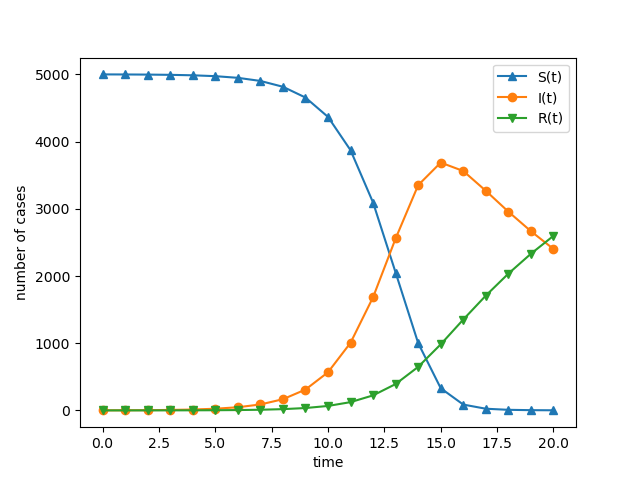
\includegraphics{Images/5000 1 0 0_0002 0_1.png}
\end{center}
\begin{flushleft}
$S_0$ = 5000;\\
$I_0$ = 1;\\
$R_0$ = 0;\\
$\beta$ = 0.0002;\\
$\gamma$ = 0.1;\\
Ta sẽ lấy trường hợp 1 làm tiêu chuẩn để so sánh và phân tích với các trường hợp khác\\
Tốc độ gia tăng số người nhiễm trong trường hợp này tăng nhanh vào từ ngày đầu đến khoảng ngày 14, với đồ thị bên trái cực đại giống với đồ thị hàm số mũ, đạt cực đại vào ngày 15 và sau đó giảm dần do số người khỏe mạnh giảm xuống 0.\\
Số người khỏe mạnh giảm dần và vào khoảng ngày 18, số người khỏe mạnh đã giảm xuống 0.


\subsubsection{Trường hợp 2}
\begin{center}
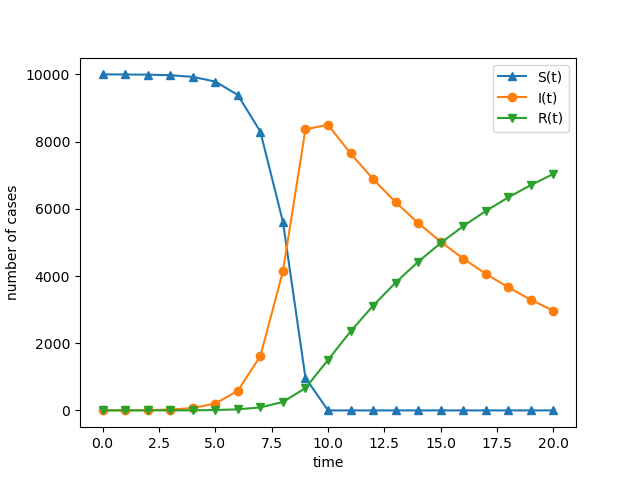
\includegraphics{Images/10000 1 0 0_0002 0_1.png}
\end{center}
\begin{flushleft}
$S_0$ = 10000 - Tăng 2 lần so với trường hợp 1;\\
$I_0$ = 1;\\
$R_0$ = 0;\\
$\beta$ = 0.0002;\\
$\gamma$ = 0.1;\\
Ta có thể thấy tốc độ gia tăng của số người bị nhiễm giảm đi rất nhiều so với trường hợp 1,đạt cực đại vào ngày 10, so với trường hợp 1 là ngày 15 và số lượng người khỏe mạnh cũng giảm nhanh hơn nhiều.\\
Số người hồi phục trong trường hợp này cũng tăng nhanh hơn so với trường hợp 1, nhưng đây cũng là kết quả từ việc số người nhiễm tăng nhanh hơn (Do số ngươi hồi phục tăng nhanh hay chậm phụ thuộc vào $\gamma$ và số người bị nhiễm)
\end{flushleft}
$\longrightarrow$ Ta có thể thấy tốc độ gia tăng số người nhiễm bện phụ thuộc rất nhiều vào số người dân, việc này trong thực tế có thể hiểu là những biện pháp cách ly, hạn chế đi lại... ở trường hợp 1 để giảm số người dân trong từng không gian kín, đã không áp dụng ở trường hợp 2 làm tăng đáng kể số người nhiễm bệnh và tốc độ lây lan của dịch. 
\end{flushleft}

\subsubsection{Trường hợp 3}
\begin{center}
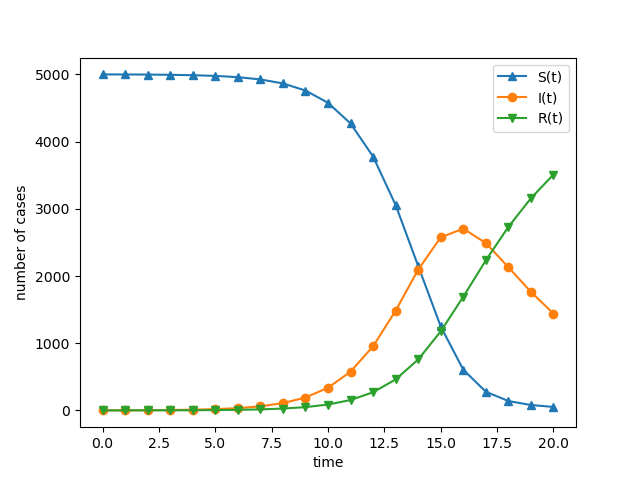
\includegraphics{Images/5000 1 0 0_0002 0_2.png}
\end{center}
\begin{flushleft}
$S_0$ = 5000;\\
$I_0$ = 1;\\
$R_0$ = 0;\\
$\beta$ = 0.0002;\\
$\gamma$ = 0.2 - Tăng 2 lần so với trường hợp 1;\\
\end{flushleft}
Với $S_0$ bằng trường hợp 1, thì ta có thể thấy 2 trường hợp 1 và 3 có số người bị nhiễm và số người khỏe mạnh có đường biểu diễn giống nhau và các phân tích ở trường hợp 1 có thể áp dụng vào trường hợp 3.\\
Sự khác biệt ở trượng hợp 1 và trường hợp 3 là ở số người hồi phục, do $\gamma$ tăng nên tốc độ của số người hồi phục tăng cũng cao hơn so với trường hợp 1.


\subsubsection{Trường hợp 4}
\begin{center}
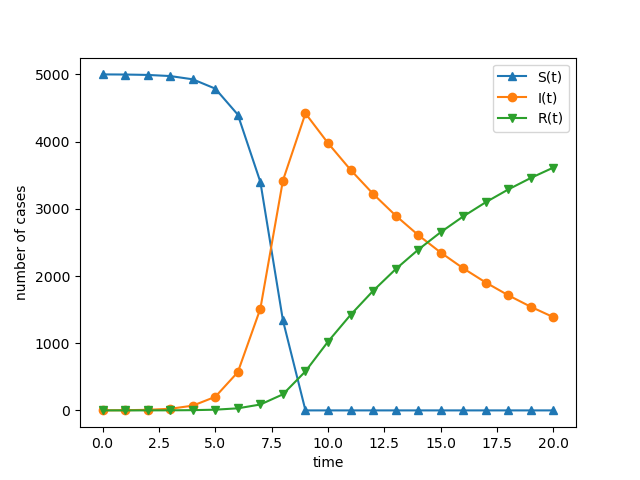
\includegraphics{Images/5000 1 0 0_0004 0_1.png}
\end{center}
\begin{flushleft}
$S_0$ = 5000;\\
$I_0$ = 1;\\
$R_0$ = 0;\\
$\beta$ = 0.0004 - Tăng 2 lần so với trường hợp 1;\\
$\gamma$ = 0.1;\\
\end{flushleft}
Số người bị nhiễm tăng nhanh hơn rất nhiều so với trường hợp 1, và tăng nhanh hơn cả trường hợp 2, đạt cực đại vào khoảng ngày 9.\\
Số người hồi phục trong trường hợp này cũng tăng nhanh hơn so với trường hợp 1, nhưng đây cũng là kết quả từ việc số người nhiễm tăng nhanh hơn (Do số ngươi hồi phục tăng nhanh hay chậm phụ thuộc vào $\gamma$ và số người bị nhiễm).\\
Số người khỏe mạnh giảm rất nhanh, và xuống 0 bào ngày 9
$\longrightarrow$ Trong thực tế, $\beta$ tăng 2 lần có thể được hiều là các cá thể trong mô hình đã không vệ sinh tốt, đeo khẩu trang nơi công cộng, ... như ở trường hợp 1, và điều này dẫn đến số người nhiễm bệnh tăng rất nhanh.


\subsubsection{Trường hợp 5}
\begin{center}
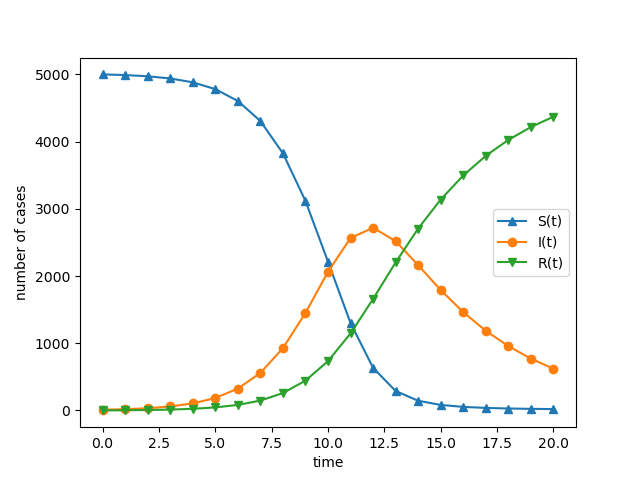
\includegraphics{Images/5000 10 0 0_0002 0_2.png}
\end{center}
\begin{flushleft}
$S_0$ = 5000;\\
$I_0$ = 10; - Tăng 10 lần so với trường hợp 1\\
$R_0$ = 0;\\
$\alpha$ = 0.0002;\\
$\beta$ = 0.2;\\
\end{flushleft}
Số người bị nhiễm tăng và số người khỏe mạnh giảm nhanh hơn so với tường hợp 1 nhưng không nhanh bằng trường hợp 4, mặc dù số người bị nhiễm ban đầu tăng gấp 10 lần
\subsection{Nhận xét}
Từ những số liệu thu được từ các trường hợp trong 3.5, ta rút ra được kết luận như sau về mô hình SIR:\\
Số người khỏe mạnh và số người bị nhiễm có liên quan chặt chẽ đến nhau, với tốc độ tăng của số người bị nhiễm sẽ làm tăng tốc độ giảm của số người khỏe mạnh, và tốc độ gia tăng của số người bị nhiễm tỷ lệ thuận với số người khỏe mạnh.\\
Số người bị nhiễm tăng nhanh khi trong cộng đồng có nhiều người khỏe mạnh,$\beta$ cao, trong đó, số người bị nhiễm tăng nhanh hay chậm phụ thuộc nhiều vào $\beta$.








\section{Bài toán 3. Lấy mẫu sử dụng thuật toán Metropolis-Hastings}
\\
Nhóm chọn ngôn ngữ thống kê R để thực hiện bài toán.\\

Mô tả cách thiết lập và chạy Metropolis-Hastings dựa trên Markov chain Monte Carlo (MCMC) trong phạm vi mô hình SIR.\\
Ví dụ code sử dụng dữ liệu Eyam.\\
\begin{lstlisting}

library(MultiBD)

data(Eyam)

print(Eyam)

printsample_size <- 177
\end{lstlisting}
\\
Tính log của phân bố xác suất số ca mắc bệnh và số người có khả năng mắc bệnh với param cho trước. Ma trận xác suất được trả về bởi $ ddb_{-}prob() $ tương ứng với giá trị $S$ từ $a$ tới $a_{0}$  và $I$ từ $0$ tới $B$.\\
$a$ là cận dưới, $B$ là cận trên.
\\
$ ddb_{-}prob() $ Function là Xác suất chuyển tiếp của một quá trình chết/ sinh - chết..\\
\lstinline{drates1} Tỉ lệ chết đi của $S$, bằng 0 vì $S$ chỉ chuyển số lượng sang cho $I$.\\
\lstinline{brates2} Mô hình không sinh thêm phần tử.\\
\lstinline{drates2} Tỉ lệ chết của $I$ là có và bằng \lstinline{alpha*b}.\\
\lstinline{trans12} Ở đây là mô hình chuyển từ trạng thái $S$ sang trạng thái $I$
\\
\begin{lstlisting}

loglik_sir <- function(param, data) {
                                            
  alpha <- exp(param[1]) # Rates must be non-negative
  beta <- exp(param[2])
  # Set-up SIR model
  drates1 <- function(a, b) { 0 }                    
  brates2 <- function(a, b) { 0 }                     
  drates2 <- function(a, b) { alpha * b }            
  trans12 <- function(a, b) { beta * a * b }          
  sum(sapply(1:(nrow(data) - 1), # Sum across all time steps k
             function(k) {
               log( # sums the logs of logs that change from T to T + 1 state
                 dbd_prob( # Compute the transition probability matrix
                   t = data$time[k + 1] - data$time[k], # Time increment
                   a0 = data$S[k], b0 = data$I[k], # From: S(t_k), I(t_k)
                   drates1, brates2, drates2, trans12,
                   a = data$S[k + 1], B = data$S[k] + data$I[k] - data$S[k + 1],
                   computeMode = 4, nblocks = 80 # Compute using 4 threads
                 )[1, data$I[k + 1] + 1] # To: S(t_(k+1)), I(t_(k+1))
               )
             }))
}
\end{lstlisting}
\\
Phân bố xác suất tiên nghiệm của số ca mắc bệnh và số ca phục hồi dựa trên phân bố chuẩn.

\\
\begin{lstlisting}
logprior <- function(param) { 
  log_alpha <- param[1]
  log_beta <- param[2]
  dnorm(log_alpha, mean = 0, sd = 100, log = TRUE) +
    dnorm(log_beta, mean = 0, sd = 100, log = TRUE)
}

library(MCMCpack)

alpha0 <- 3.39
beta0 <- 0.0212

post_sample <- MCMCmetrop1R(fun = function(param) { loglik_sir(param, Eyam) + logprior(param) },
                            theta.init = log(c(alpha0, beta0)),
                            mcmc = 177, burnin = 50)
# Sampling of beta, gamm

\end{lstlisting}
\\
Vẽ đồ thị minh họa:
\\
\begin{lstlisting}
plot(as.vector(post_sample[,1]), type = "l", xlab = "Iteration", ylab = expression(log(alpha)))

plot(as.vector(post_sample[,2]), type = "l", xlab = "Iteration", ylab = expression(log(beta)))


R_0 <- 0 
for(i in 1:8){
   R_0 <- R_0 + exp(loglik_sir(c(post_sample[i,1], post_sample[i,2]), Eyam))*(exp(post_sample[i,1])/exp(post_sample[i,2]))
}

print(R_0)




\end{lstlisting}

\\


\begin{center}
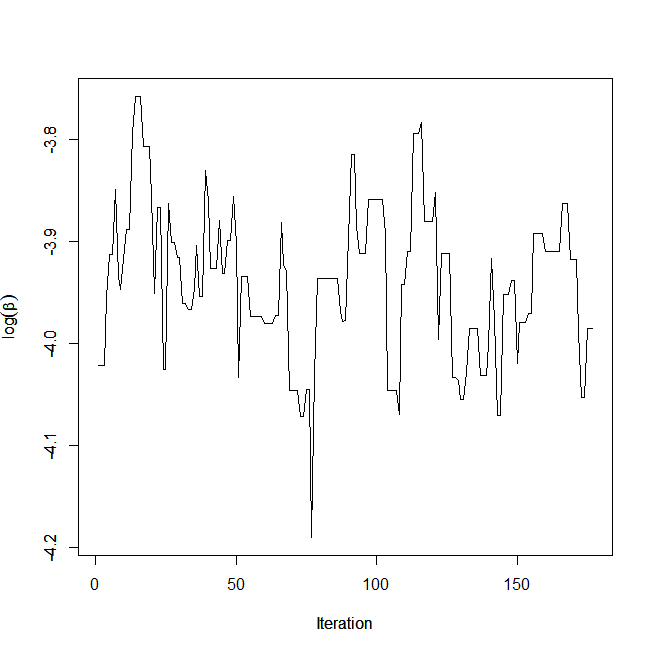
\includegraphics[scale=.5]{Images/Sir1.png}

\end{center}


Kết quả tính được với ví dụ trên là :
\lstinline{The Metropolis acceptance rate was 0.51542}\\


\section{Bài toán 4. Tìm hệ số $R0$ của khu vực tự chọn}
...
\section{Nhật ký công việc - Log Assignment}
Tuần 1:  \\ 


% Please add the following required packages to your document preamble:
% \usepackage[table,xcdraw]{xcolor}
% If you use beamer only pass "xcolor=table" option, i.e. \documentclass[xcolor=table]{beamer}
\begin{table}[h]
\begin{tabular}{|l|l|l|l|}
\hline
{\color[HTML]{010066} \textbf{Thời gian}} & {\color[HTML]{010066} \textbf{Địa điểm}}                                            & {\color[HTML]{010066} \textbf{Nội dung công việc}}                                              & {\color[HTML]{010066} \textbf{Kết quả}}                                                                    \\ \hline
Thứ 5( 02/07/2020)                        & \begin{tabular}[c]{@{}l@{}}Tại thư viện H1\\ trường ĐH Bách khoa\\ tpHCM\end{tabular} & Tìm hiểu đề tài bài tập lớn                                                                     & \begin{tabular}[c]{@{}l@{}}Hiểu được tổng quan\\ yêu cầu bài tập lớn\end{tabular}                          \\ \hline
Thứ 7( 04/07/2020)                        & \begin{tabular}[c]{@{}l@{}}Tại thư viện H1\\ trường ĐH Bách khoa\\ tpHCM\end{tabular} & \begin{tabular}[c]{@{}l@{}}Tìm hiểu ngôn ngữ R,\\  ngôn ngữ Python, mô \\ hình SIR\end{tabular} & \begin{tabular}[c]{@{}l@{}}Hiểu được tổng quan \\ và cách làm việc cơ bản \\ với các ngôn ngữ\end{tabular} \\ \hline
\end{tabular}
\end{table}

Tuần 2:  \\ 
% Please add the following required packages to your document preamble:
% \usepackage[table,xcdraw]{xcolor}
% If you use beamer only pass "xcolor=table" option, i.e. \documentclass[xcolor=table]{beamer}
\begin{table}[h]
\begin{tabular}{|l|l|l|l|}
\hline
{\color[HTML]{010066} \textbf{Thời gian}} & {\color[HTML]{010066} \textbf{Địa điểm}}                                               & {\color[HTML]{010066} \textbf{Nội dung công việc}}                                                    & {\color[HTML]{010066} \textbf{Kết quả}}                                                     \\ \hline
Thứ 4( 08/07/2020)                        & \begin{tabular}[c]{@{}l@{}}Tại thư viện H1\\ trường ĐH Bách khoa \\ tpHCM\end{tabular} & \begin{tabular}[c]{@{}l@{}}Tạo git làm việc nhóm,\\ phân chia công việc\end{tabular}                  & \begin{tabular}[c]{@{}l@{}}Hiểu được các bước \\ tiến hành của bài tập lớn\end{tabular}     \\ \hline
Thứ 7( 11/07/2020)                        & \begin{tabular}[c]{@{}l@{}}Tại thư viện H1\\ trường ĐH Bách khoa\\ tpHCM\end{tabular}  & \begin{tabular}[c]{@{}l@{}}Trao đổi các phần của \\ mô hình , thảo luận \\ tìm giải pháp\end{tabular} & \begin{tabular}[c]{@{}l@{}}Hỗ trợ nhau thực hiện các \\ phần việc đã phân công\end{tabular} \\ \hline
\end{tabular}
\end{table}

Tuần 3: \\
% Please add the following required packages to your document preamble:
% \usepackage[table,xcdraw]{xcolor}
% If you use beamer only pass "xcolor=table" option, i.e. \documentclass[xcolor=table]{beamer}
\begin{table}[h]
\begin{tabular}{|l|l|l|l|}
\hline
{\color[HTML]{010066} \textbf{Thời gian}} & {\color[HTML]{010066} \textbf{Địa điểm}}                                               & {\color[HTML]{010066} \textbf{Nội dung công việc}}                                & {\color[HTML]{010066} \textbf{Kết quả}}                                                                                              \\ \hline
Thứ 4( 15/07/2020)                        & \begin{tabular}[c]{@{}l@{}}Tại thư viện H1\\ trường ĐH Bách khoa \\ tpHCM\end{tabular} & \begin{tabular}[c]{@{}l@{}}Kiểm tra tiến độ \\ công việc\end{tabular}             & \begin{tabular}[c]{@{}l@{}}Các thành viên tiến triển\\ công việc đúng yêu cầu\end{tabular}                                           \\ \hline
Thứ 7( 18/07/2020)                        & \begin{tabular}[c]{@{}l@{}}Tại thư viện H1\\ trường ĐH Bách khoa\\ tpHCM\end{tabular}  & \begin{tabular}[c]{@{}l@{}}Kiểm tra tiến độ\\ công việc\end{tabular}              & \begin{tabular}[c]{@{}l@{}}Hoàn thành cơ sở \\ lý thuyết, bài 1,2 và 3.\\ Bài 4 gặp khó khăn trong\\ việc xử lý số liệu\end{tabular} \\ \hline
Chủ Nhật(19/07/2020)                      & \begin{tabular}[c]{@{}l@{}}Tại thư viện H1\\ trường ĐH Bách khoa\\ tpHCM\end{tabular}  & \begin{tabular}[c]{@{}l@{}}Thảo luận, tìm kiếm\\ giải pháp cho bài 4\end{tabular} & \begin{tabular}[c]{@{}l@{}}Giải quyết được bài 4,\\ tuy chưa là cách tốt nhất\end{tabular}                                           \\ \hline
\end{tabular}
\end{table}

Tuần 4:\\
% Please add the following required packages to your document preamble:
% \usepackage[table,xcdraw]{xcolor}
% If you use beamer only pass "xcolor=table" option, i.e. \documentclass[xcolor=table]{beamer}
\begin{table}[h]
\begin{tabular}{|l|l|l|l|}
\hline
{\color[HTML]{010066} \textbf{Thời gian}} & {\color[HTML]{010066} \textbf{Địa điểm}}                                               & {\color[HTML]{010066} \textbf{Nội dung công việc}}                           & {\color[HTML]{010066} \textbf{Kết quả}}                                       \\ \hline
Thứ 3( 21/07/2020)                        & \begin{tabular}[c]{@{}l@{}}Tại thư viện H1\\ trường ĐH Bách khoa \\ tpHCM\end{tabular} & \begin{tabular}[c]{@{}l@{}}Tổng kết bài tập lớn\\ -viết báo cáo\end{tabular} & \begin{tabular}[c]{@{}l@{}}Hoàn thành 4/5\\ bài toán bài tập lớn\end{tabular} \\ \hline
\end{tabular}
\end{table}

Phân chia công việc: \\
\\
\\
\\
\\
\\
\\
\\
\\
\\


\begin{table}[h]
\begin{tabular}{|l|l|l|}
\hline
{\color[HTML]{010066} \textbf{Họ tên}} & {\color[HTML]{010066} \textbf{Phân công công việc}}                                          & {\color[HTML]{010066} \textbf{Đánh giá}} \\ \hline
Lê Hồng Phong                          & \begin{tabular}[c]{@{}l@{}}Xây dựng mô hình SIR\\ + Bài 3\end{tabular}                       & 95\%                                     \\ \hline
Tăng Minh Nhật                         & \begin{tabular}[c]{@{}l@{}}Xây dựng mô hình SIR\\ + Bài 4\end{tabular}                       & 100\%                                    \\ \hline
Đặng Thành Ngân                        & \begin{tabular}[c]{@{}l@{}}Tổng hợp lý thuyết về \\ xác suất thống kê+ \\ Bài 4\end{tabular} & 95\%                                     \\ \hline
Đỗ Lê Thiên Ân                         & \begin{tabular}[c]{@{}l@{}}Lý thuyết thuật toán Metropolis-\\ Hastings +Bài 2\end{tabular}   & 90\%                                     \\ \hline
Huỳnh Thiên Trình                      & \begin{tabular}[c]{@{}l@{}}Lý thuyết phương pháp xấp xỉ Euler\\ + Bài 3\end{tabular}         & 95\%                                     \\ \hline
\end{tabular}
\end{table}
\\
\\
\\
\\


\section{Kết luận}



%%%%%%%%%%%%%%%%%%%%%%%%%%%%%%%%%
\addcontentsline{toc}{section}{Tài liệu}
\begin{thebibliography}{99999}
\bibitem{Atkinson} 
Atkinson, Kendall A.
\textit{(1989), An Introduction to Numerical Analysis (ấn bản 2), New
York: John Wiley \& Sons}. 

\bibitem{Butcher} 
Butcher, John C.
\textit{(2003), Numerical Methods for Ordinary Differential Equations, New
York: John Wiley \& Sons}. 

\bibitem{Chien Dang} 
Tính toán khoa học - Chương 6: Bài toán giá trị ban đầu với phương trình vi phân thông thường
\textit{by Chien Dang on www.slideshare.net}. 

\end{thebibliography}
\end{document}
